\chapter{Kalman Filter design for our robot}
Since the 16 MHz CPU on the MEGA2560 board was not able to carry out all the matrix calculations required by the Kalman filter at 100 Hz, we have decided to do all the computations host-side using the 2.7 GHz CPU on our PC\footnote{PC stands for Portable Computer} and send the observations via UART from the robot at 100 Hz.\\

In order to use the Kalman filter presented in the previous chapter, we only have to decide how to model our problem. More in detail we must:
\begin{itemize}
	\item choose how to represent the state,
	\item choose how to represent the controls,
	\item implement a transition model,
	\item choose how to represent the observations,
	\item implement an observation model.
\end{itemize}

Our implementation of the filter is shown in Appendix \ref{kf_implementation}.

\section{Predict phase}

\subsection{State vector}\label{state}
Our state must represent all the information on the position and orientation of the robot. Therefore we have used an 8-components state:
\begin{itemize}
	\item x representing the global displacement along the x-axis,
	\item $\dot{x}$ representing the translational velocity along the global x-axis,
	\item $\ddot{x}$ representing the translational acceleration along the global x-axis,
	\item y representing the global displacement along the y-axis,
	\item $\dot{y}$ representing the translational velocity along the global y-axis,
	\item $\ddot{y}$ representing the translational acceleration along the global y-axis,
	\item $\theta$ representing the global orientation along the z-axis,
	\item $\dot{\theta}$ representing the rotational velocity along the global z-axis.
\end{itemize}
We have included the translational accelerations because our accelerometers measure accelerations, instead we have stopped to rotational velocities because this is what our gyroscope measures.\\

Since our state will be represented by a Gaussian distribution we need to initialize both its mean and its covariance. We have decided to initialize them both with zeros because we want to measure the displacement from the starting position and because there is no uncertainty at the beginning.

\subsection{Controls vector}\label{controls}
Since our robot is pushed by hand (having no motors), we have no knowledge about the controls vector. However we will use this vector to model noise in the transition process and to introduce uncertainty in it; therefore we will assume the control vector to be zero-mean but with non-zero covariance.\\

We will use the controls vector to model spikes in the translational accelerations or in the rotational velocity which could not be observed.
\begin{itemize}
	\item $\dddot{x}$ representing a derivative of the translational acceleration along the global x-axis,
	\item $\dddot{y}$ representing a derivative of the translational acceleration along the global y-axis,
	\item $\ddot{\theta}$ representing a derivative of the rotational velocity (i.e. a rotational acceleration) along the global z-axis.
\end{itemize}

We will use the following covariance matrix:
\begin{align}
	\Sigma_u = \begin{pmatrix}
				0.1 & 0 & 0\\
				0 & 0.1 & 0\\
				0 & 0 & 0.5\\
			\end{pmatrix}
\end{align}

We need high control covariances because, since we are pushing the robot by hand, our process is very noisy; surely if we had engines controlling the robot's wheels the process would be more continuous and we could use lower covariances.

\subsection{Transition model}
We are now ready to implement the transition model, which will be used in the Predict phase. In order to define the affine transformation \ref{pred_model}, we must define the state transition matrix $A_t$ and the input matrix $B_t$.\\

According to how we defined the state in section \ref{state} and to some basics of kinematics\footnote{Basic kinematic relationships between position, velocity and acceleration:\begin{fleqn}\begin{equation}x = x + \dot{x} \Delta t + .5 \ddot{x} \Delta t^2\nonumber\end{equation}\begin{equation}\dot{x} = \dot{x} + \ddot{x} \Delta t\nonumber\end{equation}\end{fleqn}}, we can define the following state transition matrix:
\begin{align}
	A = \begin{pmatrix}
				1 & \Delta t & .5 \Delta t^2 & 0 & 0 & 0 & 0 & 0\\
				0 & 1 & \Delta t & 0 & 0 & 0 & 0 & 0\\
				0 & 0 & 1 & 0 & 0 & 0 & 0 & 0\\
				0 & 0 & 0 & 1 & \Delta t & .5 \Delta t^2 & 0 & 0\\
				0 & 0 & 0 & 0 & 1 & \Delta t & 0 & 0\\
				0 & 0 & 0 & 0 & 0 & 1 & 0 & 0\\
				0 & 0 & 0 & 0 & 0 & 0 & 1 & \Delta t\\
				0 & 0 & 0 & 0 & 0 & 0 & 0 & 1\\
			\end{pmatrix}
\end{align}

According to how we have defined the controls vector in section \ref{controls} we can define the following input matrix:
\begin{align}
	B = \begin{pmatrix}
				.167 \Delta t^3 & 0 & 0\\
				.5 \Delta t^2 & 0 & 0\\
				\Delta t & 0 & 0\\
				0 & .167 \Delta t^3 & 0\\
				0 & .5 \Delta t^2 & 0\\
				0 & \Delta t & 0\\
				0 & 0 & .167 \Delta t^3\\
				0 & 0 & .5 \Delta t^2\\
				0 & 0 & \Delta t\\
			\end{pmatrix}
\end{align}

We can notice how this two matrices are independent of the precise current sampling instant and they remain constant throughout all the computation.\\

From the equations \ref{pred_mean} and \ref{pred_cov}, remembering that our control is zero-mean we obtain the following predict phase equations:
\begin{align}
	\mu_{t|t-1} &= A \mu_{t-1|t-1}\\
	\Sigma_{t|t-1} &= A \Sigma_{t-1|t-1} A^T + B \Sigma_{u,t-1} B^T
\end{align}


\section{Update phase}
\subsection{IMU observations}
\subsubsection{IMU observations vector}
The accelerometer gives us measurements about the accelerations along the three axes, while the gyroscope measures rotational velocities along the three axes. Assuming that our robot moves only in 2D we will consider only:
\begin{itemize}
	\item $\ddot{x}_z$ which is the translational acceleration along the x-axis measured by the accelerometer,
	\item $\ddot{y}_z$ which is the translational acceleration along the y-axis measured by the accelerometer,
	\item $\dot{\theta}_z$ which is the rotational velocity along the z-axis measured by the gyroscope.
\end{itemize}

We will consider these measurements as independent, therefore the IMU covariance matrix will be diagonal. Moreover since the accelerometer is very noisy and inaccurate, we will give the accelerometer observations a relevant covariance, instead since the gyroscope is much less noisy we will give it less covariance.
\begin{align}
	\Sigma_{IMU} = \begin{pmatrix}
				0.1 & 0 & 0\\
				0 & 0.1 & 0\\
				0 & 0 & 0.000001\\
			\end{pmatrix}
\end{align}
Let us note how the measurement error covariances were defined by trial and error since they were not provided by the IMU manufacturer.

\subsubsection{IMU observation model}
To define the observation model for the IMU observations, we must define only the observation matrix $C_t$ to be used in the equation \ref{upd_model}.
\begin{align}
	C_{IMU} = \begin{pmatrix}
				0 & 0 & 1 & 0 & 0 & 0 & 0 & 0\\
				0 & 0 & 0 & 0 & 0 & 1 & 0 & 0\\
				0 & 0 & 0 & 0 & 0 & 0 & 0 & 1\\
			\end{pmatrix}
\end{align}



\subsection{Encoders observations}
Unlike the IMU which gives us measurements for which the definition of an observation matrix is immediate, the encoders measures the wheel rotations.\\

\subsubsection{Linearized Observation Matrix}
We have started considering the wheels rotations as the observations to be used in Kalman filter. Since we assume the encoders to be very accurate we assumed these measurements to have small covariance.
\begin{align}
	\Sigma_{encoders,linearized} = \begin{pmatrix}
				0.0000001 & 0\\
				0 & 0.0000001\\
			\end{pmatrix}
\end{align}
Let us note how these measurement error covariances were defined by trial and error since they were not provided by the encoders manufacturer.

\begin{figure}[!ht]
	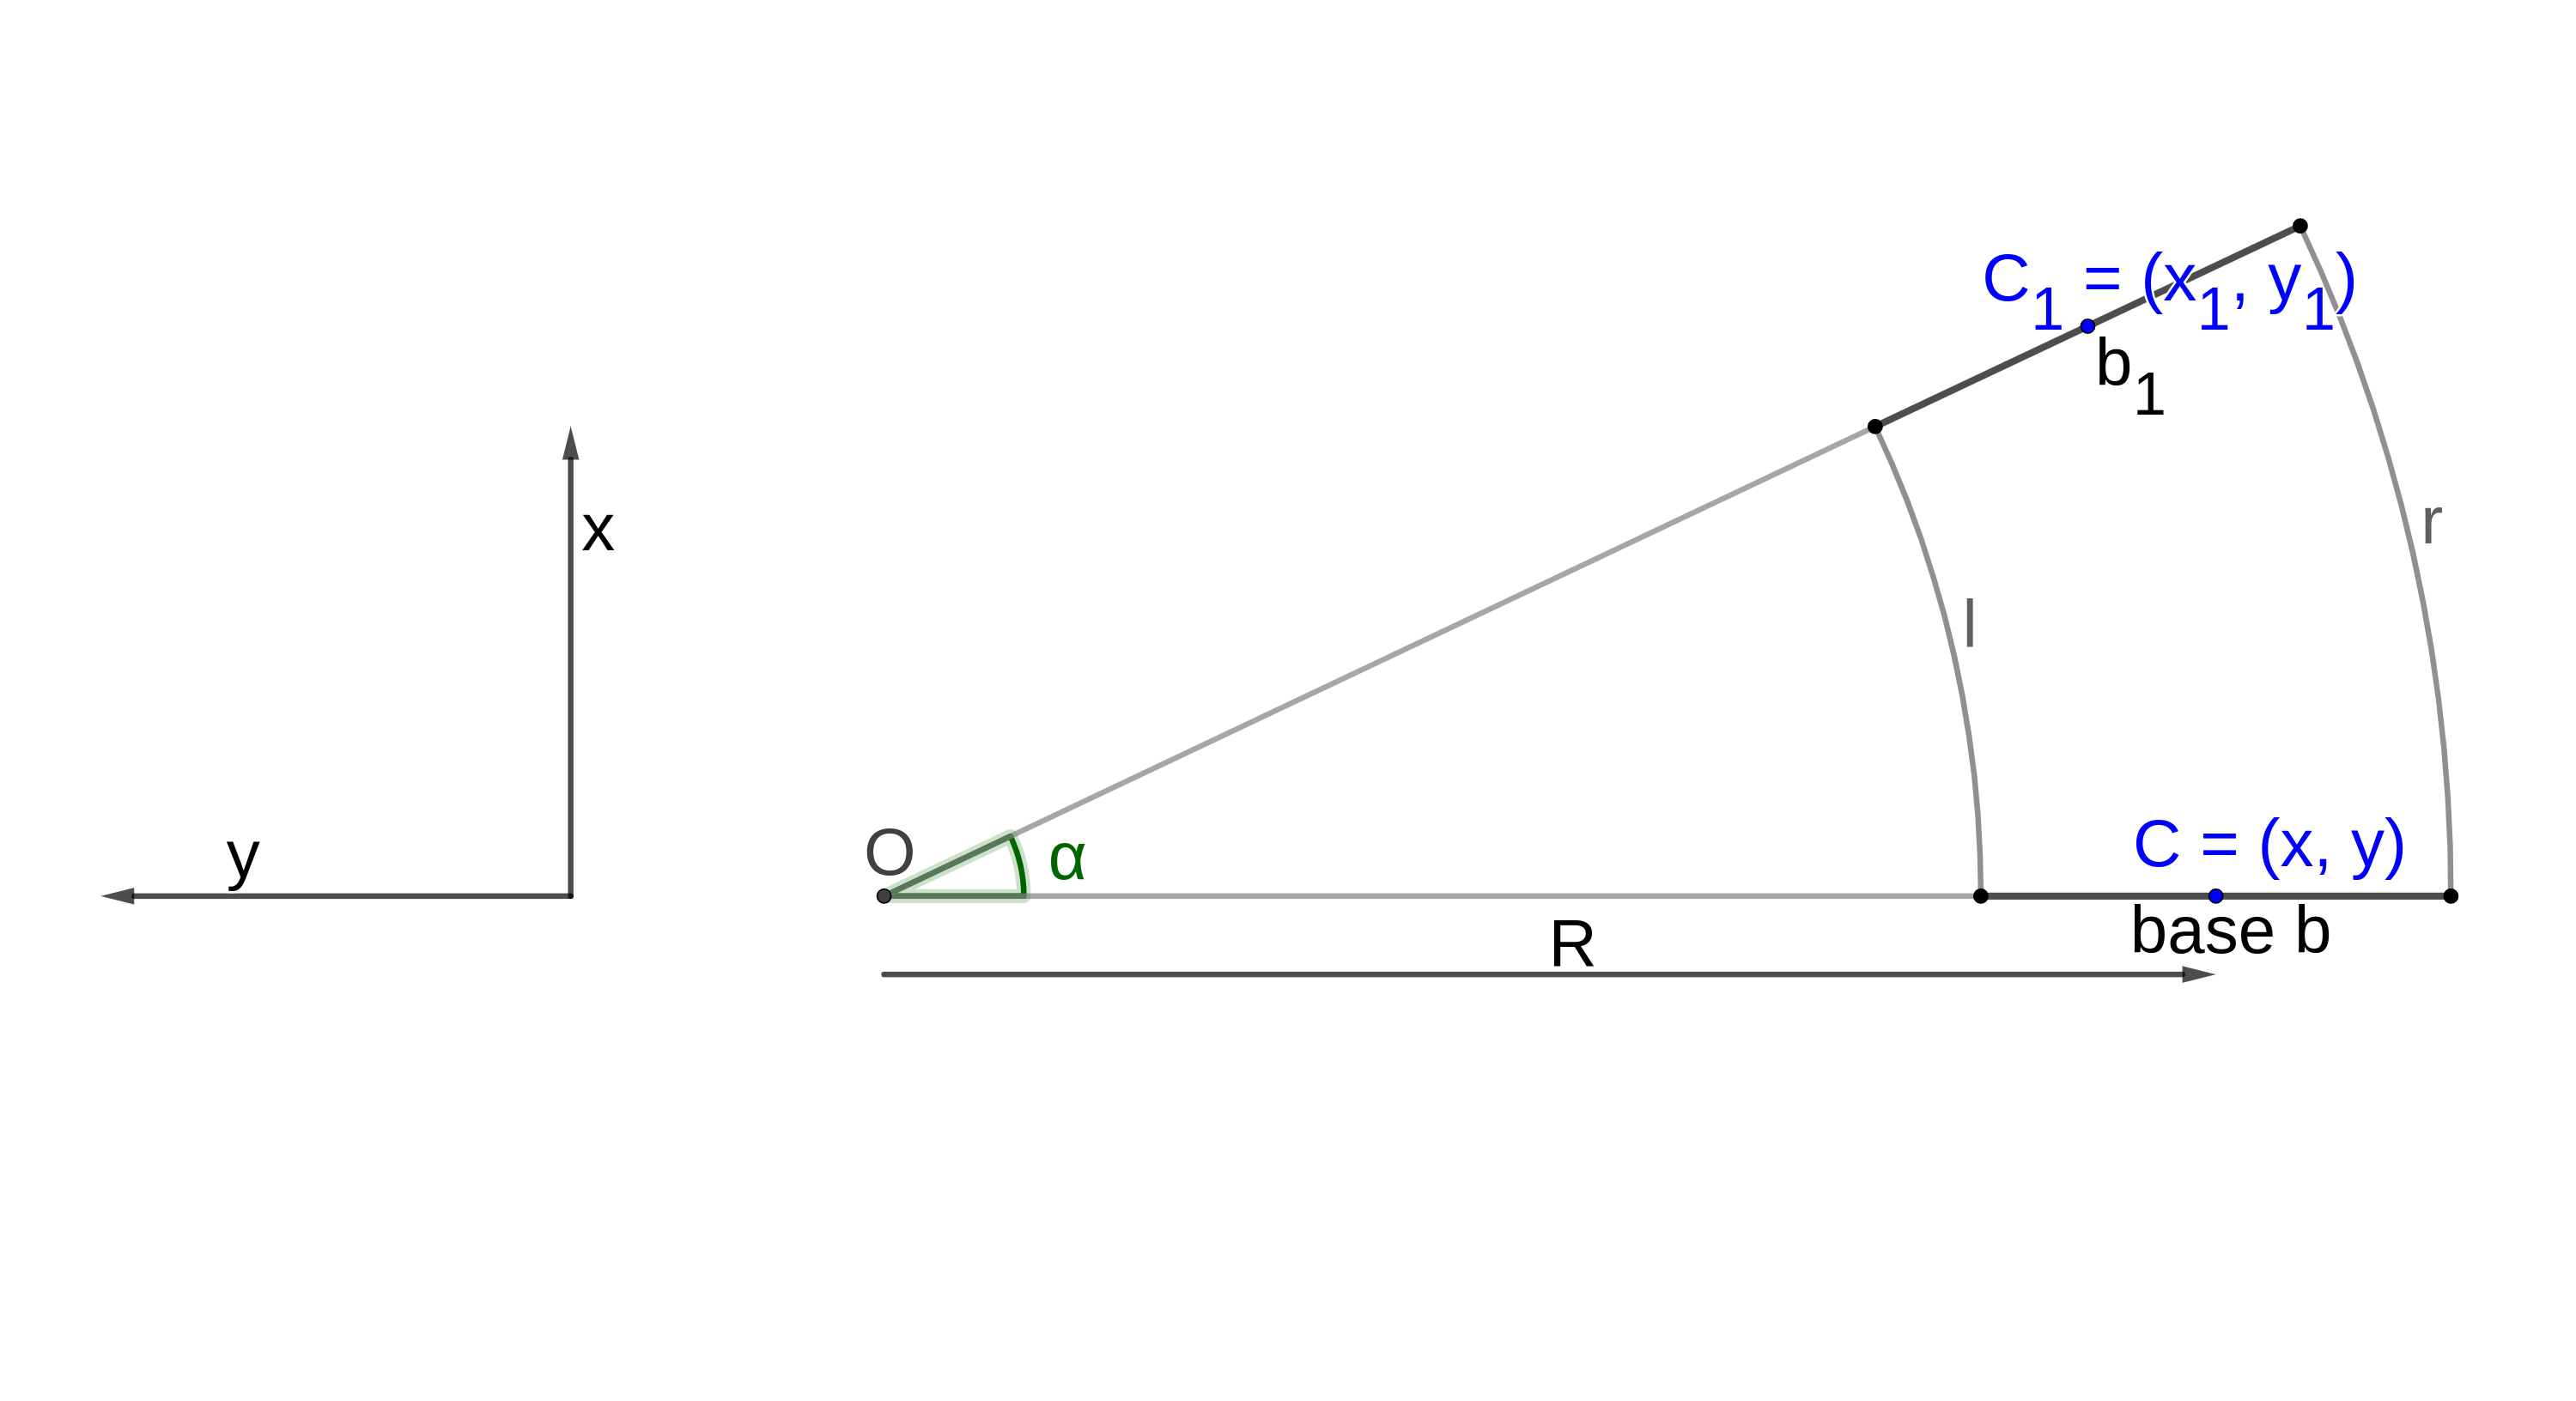
\includegraphics[scale=0.9]{differential_drive_1}
	\captionsetup{justification=centering, margin=1.5cm}
	\centering
	\caption{Model of an instantaneous movement through a rotation.}
	\centering
\end{figure}

As described in my thesis\supercite{Graziano:BscThesis:2019}, the rotations of the left and right wheel (\textit{l} and \textit{r} respectively) are related to the parameters of the local rotation (the radius \textit{R} and the angle $\Delta \theta$) by the equations (where \textit{b} is the length of the wheel axis):
\begin{align}
	r &= (R + b/2) \Delta \theta\label{r}\\
	l &= (R - b/2) \Delta \theta\label{l}
\end{align}

Moreover \textit{R} is related to the local movement by the equation:
\begin{align}
	\Delta x_{local} = R \sin\Delta \theta\label{x_local_r}
\end{align}

and the local movement can be related to the global movement using:
\begin{align}
	\Delta x_{local} = \Delta x \cos\theta + \Delta y \sin\theta\label{x_local_global}
\end{align}

Therefore using the \ref{x_local_r} and the \ref{x_local_global}:
\begin{align}
	R = \frac{\Delta x_{local}}{\sin\Delta \theta} = \frac{\Delta x \cos\theta + \Delta y \sin\theta}{\sin\Delta \theta}\label{R}
\end{align}

Finally using the \ref{r}, the \ref{l} and the \ref{R}:
\begin{align}
	r &= (\frac{\Delta x \cos\theta + \Delta y \sin\theta}{\sin\Delta \theta} + b/2) \Delta \theta\\
	l &= (\frac{\Delta x \cos\theta + \Delta y \sin\theta}{\sin\Delta \theta} - b/2) \Delta \theta
\end{align}

These equations enable us to calculate the observations starting from the state, however these equations are not linear. Therefore we have linearized them using the Taylor expansion to the first order centered in zero\footnote{The Taylor expansion to the first order for a function $f(x,y)$ results in the polynomial:\begin{gather*}P = f(0,0) + \der{f(0,0)}{x} x + \der{f(0,0)}{y} y\end{gather*}}.
\begin{align}
	r &= \cos\theta \Delta x + \sin\theta \Delta y + \frac{b}{2}\Delta \theta\label{r_lin}\\
	l &= \cos\theta \Delta x + \sin\theta \Delta y - \frac{b}{2}\Delta \theta\label{l_lin}
\end{align}

In order to use these equations in the observation matrix we must write $\Delta x$, $\Delta y$, $\Delta \theta$ as a function of the state:
\begin{align}
	\Delta x &= \dot{x} \Delta t + \frac{1}{2} \ddot{x} \Delta t\label{dx}\\
	\Delta y &= \dot{y} \Delta t + \frac{1}{2} \ddot{y} \Delta t\label{dy}\\
	\Delta \theta &= \dot{\theta} \Delta t\label{dtheta}
\end{align}

Using the \ref{r_lin}, the \ref{l_lin}, the \ref{dx}, the \ref{dy} and the \ref{dtheta}:
\begin{align}
	r &= (\cos\theta \Delta t)\dot{x} + (.5 \cos\theta \Delta t^2)\ddot{x} + (\sin\theta \Delta t)\dot{y} + (.5 \sin\theta \Delta t^2)\ddot{y} + (.5 b \Delta t)\dot{\theta}\\
	l &= (\cos\theta \Delta t)\dot{x} + (.5 \cos\theta \Delta t^2)\ddot{x} + (\sin\theta \Delta t)\dot{y} + (.5 \sin\theta \Delta t^2)\ddot{y} - (.5 b \Delta t)\dot{\theta}
\end{align}

Now we are ready to write the linearized observation matrix:
\begin{align}
	C_{encoders,linearized} = \begin{pmatrix}
				0 & \cos\theta \Delta t & .5 \cos\theta \Delta t^2 & 0 & \sin\theta \Delta t & .5 \sin\theta \Delta t^2 & 0 & .5 b \Delta t\\
				0 & \cos\theta \Delta t & .5 \cos\theta \Delta t^2 & 0 & \sin\theta \Delta t & .5 \sin\theta \Delta t^2 & 0 & -.5 b \Delta t\\
			\end{pmatrix}
\end{align}

However in this matrix all the dependencies from $y$, $\dot{y}$, $\ddot{y}$ are functions of $\sin\theta$. Since we start with our robot in motionless state with orientation corresponding to $\theta = 0$ (and since $\sin 0 = 0$), we will have zero components in the observation matrix for all the components relative to the motion along the y-axis, therefore the update phase will not reduce the uncertainty relative to these components as it does for the ones relative to the motion along the x-axis. This leads to high uncertainty on the y-axis even if the robot is stationary and we observe no wheel rotations. This is certainly a non-desirable effect.

\subsubsection{Converted Measurements Observation Matrix}
In order to solve the problem previously described, we have changed our approach to the encoders measurements. This time we have not considered as observations directly the wheel rotations, but we converted the wheel rotations in the local instant movement and used this movement as the observation.\\

As described in my thesis\supercite{Graziano:BscThesis:2019} we can calculate the local movement using the Differential Drive technique:
\begin{align}
	\Delta x &= \frac{r + l}{2} \frac{\sin \Delta\theta}{\Delta\theta}\\
	\Delta y &= \frac{r + l}{2} \frac{1 - \cos \Delta\theta}{\Delta\theta}\\
	\Delta\theta &= \frac{r - l}{b}
\end{align}

Since we assume the encoders to be very accurate, we can still believe these observations as reliable. However we must point out that the encoders are subject to errors when the wheels start to slip; in this case the highest drift will be seen in the orientation because calculating $\Delta x$, $\Delta y$ we use the mean between \textit{r} and \textit{l} while updating $\Delta\theta$ we use the difference between the two wheels rotations. Therefore we will give a slightly higher covariance to $\Delta\theta$.
\begin{align}
	\Sigma_{encoders,converted} = \begin{pmatrix}
				0.0000001 & 0 & 0\\
				0 & 0.0000001 & 0\\
				0 & 0 & 0.000001
			\end{pmatrix}
\end{align}

Using the local movement $\Delta\theta$, $\Delta x$, $\Delta y$ as the observation, we can define the observation matrix as follows.
\begin{align}
	\Delta x_{local} &= \Delta x \cos\theta + \Delta y \sin\theta\\
	\Delta y_{local} &= -\Delta x \sin\theta + \Delta y \cos\theta\\
	\Delta\theta_{local} &= \Delta\theta
\end{align}

Using again the \ref{dx}, the \ref{dy} and the \ref{dtheta}, we can rewrite the previous equations as follows:
\begin{align}
	\Delta x_{local} &= (\cos\theta \Delta t)\dot{x} + (.5 \cos\theta \Delta t^2)\ddot{x} + (\sin\theta \Delta t)\dot{y} + (.5 \sin\theta \Delta t^2)\ddot{y}\\
	\Delta y_{local} &= (-\sin\theta \Delta t)\dot{x} + (-.5 \sin\theta \Delta t^2)\ddot{x} + (\cos\theta \Delta t)\dot{y} + (.5 \cos\theta \Delta t^2)\ddot{y}\\
	\Delta\theta_{local} &= \dot{\theta} \Delta t
\end{align}
Finally we can write the converted measurements observation matrix:
\begin{align}
	C_{encoders,converted} = \begin{pmatrix}
				0 & \cos\theta \Delta t & .5 \cos\theta \Delta t^2 & 0 & \sin\theta \Delta t & .5 \sin\theta \Delta t^2 & 0 & 0\\
				0 & -\sin\theta \Delta t & -.5 \sin\theta \Delta t^2 & 0 & \cos\theta \Delta t & .5 \cos\theta \Delta t^2 & 0 & 0\\
				0 & 0 & 0 & 0 & 0 & 0 & 0 & \Delta t\\
			\end{pmatrix}
\end{align}

\subsection{Joint Update phase}
Since we are sampling both the sensors at the same rate (100 Hz), we will consider a single observation vector:
\begin{itemize}
	\item $\ddot{x}_z$ which is the translational acceleration along the x-axis measured by the accelerometer,
	\item $\ddot{y}_z$ which is the translational acceleration along the y-axis measured by the accelerometer,
	\item $\dot{\theta}_z$ which is the rotational velocity along the z-axis measured by the gyroscope,
	\item $\Delta x_{local}$ which is the local displacement along the x-axis calculated from the encoders rotations,
	\item $\Delta y_{local}$ which is the local displacement along the y-axis calculated from the encoders rotations,
	\item $\Delta \theta_{local}$ which is the local orientation change calculated from the encoders rotations.
\end{itemize}

Globally the observation covariance will be:
\begin{align}
	\Sigma_z = \begin{pmatrix}
				0.1 & 0 & 0 & 0 & 0 & 0\\
				0 & 0.1 & 0 & 0 & 0 & 0\\
				0 & 0 & 0.000001 & 0 & 0 & 0\\
				0 & 0 & 0 & 0.0000001 & 0 & 0\\
				0 & 0 & 0 & 0 & 0.0000001 & 0\\
				0 & 0 & 0 & 0 & 0 & 0.000001\\
			\end{pmatrix}
\end{align}
and the observation matrix will be:
\begin{align}
	C_t = \begin{pmatrix}
				0 & 0 & 1 & 0 & 0 & 0 & 0 & 0\\
				0 & 0 & 0 & 0 & 0 & 1 & 0 & 0\\
				0 & 0 & 0 & 0 & 0 & 0 & 0 & 1\\
				0 & \cos\theta \Delta t & .5 \cos\theta \Delta t^2 & 0 & \sin\theta \Delta t & .5 \sin\theta \Delta t^2 & 0 & 0\\
				0 & -\sin\theta \Delta t & -.5 \sin\theta \Delta t^2 & 0 & \cos\theta \Delta t & .5 \cos\theta \Delta t^2 & 0 & 0\\
				0 & 0 & 0 & 0 & 0 & 0 & 0 & \Delta t\\
			\end{pmatrix}
\end{align}
We can notice how this matrix depends on the current sampling instant, in particular it depends on the current orientation. Therefore we will need to recalculate the observation matrix at each iteration of the filter.
